\documentclass[tikz,border=2]{standalone}
%% \usepackage{amsfonts}
\usepackage{lmodern} % enhanced version of computer modern
\usepackage[T1]{fontenc} % for hyphenated characters
\usepackage{amssymb}
\usepackage{amsmath}
\usepackage{amsthm}
%
\usetikzlibrary{decorations.pathreplacing,shadows,arrows,shapes,positioning,calc,backgrounds,fit}
\newcommand{\mA}{\mathcal{A}}
\newcommand{\mB}{\mathcal{B}}
\newcommand{\mC}{\mathcal{C}}
\newcommand{\mI}{\mathcal{I}}
\newcommand{\mN}{\mathcal{N}}
\newcommand{\mP}{\mathcal{P}}
\newcommand{\mR}{\mathcal{R}}
\newcommand{\mS}{\mathcal{S}}
\newcommand{\mY}{\mathcal{Y}}
% Define the layers to draw the diagram
%
\begin{document}
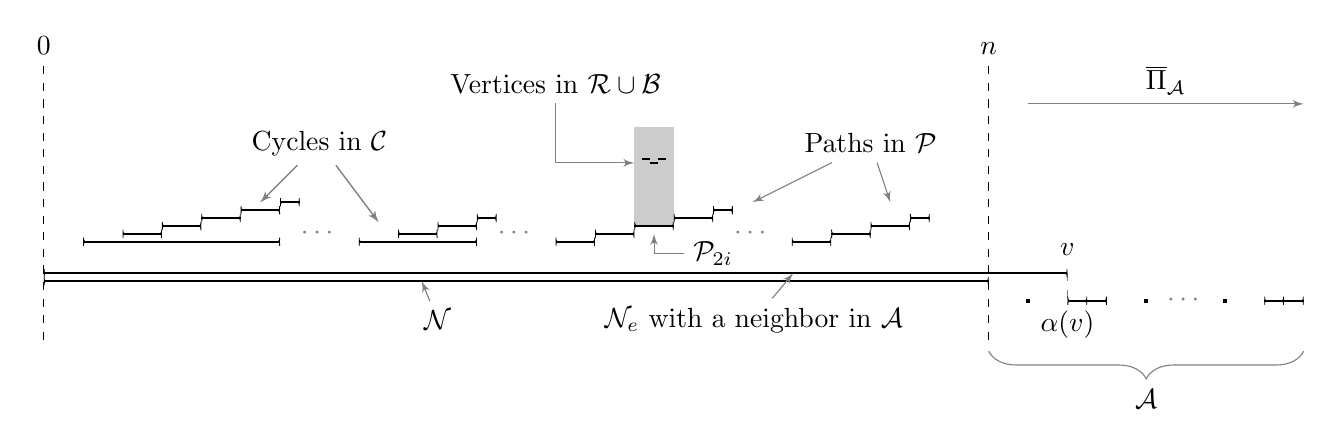
\begin{tikzpicture}
[node distance=1cm,
interval/.style={thick,>=serif cm,rounded corners=1.24pt},
uint/.style={shape=rectangle,draw=black,inner sep=.5pt,fill},
dedge/.style={gray,>=latex', shorten >=.0pt, shorten <=.0pt},
myedge/.style={thick}]
%%
% boundaries
%%
\node (0) at (0,0){};
\node (n) at (12,0){};
\draw[dashed] (0)+(0,-1.5) -- +(0,2) node[above] {$0$};
\draw[dashed] (n)+(0,-1.5) -- +(0,2) node[above] {$n$};
%%
% A
%%
\path (n) ++(0,-1) 
++(.5,0) node[uint] {}
++(.5,0) edge[interval,<->] +(.25,0) node[below,black] {$\alpha(v)$}
++(.5,0) edge[interval,<-] +(-.25,0)
++(.5,0) node[uint] {}
++(.5,0) node[gray] {$\cdots$}
++(.5,0) node[uint] {}
++(.5,0) edge[interval,<->] +(.25,0)
++(.5,0) edge[interval,<-] +(-.25,0);
\draw [gray,decorate,decoration={brace,amplitude=10pt,mirror,raise=4pt},yshift=0pt]
(n)++(0,-1.5) -- +(4,0) node [midway,below,yshift=-.5cm,black] {$\mA$};
\draw [dedge,->] (n)++(.5,1.5) -- +(3.5,0) node [black,midway,above]
{$\overline{\Pi}_{\mA}$};
%%
% N
%%
\path (0)++(0,-.75) node (Nref){}
+(0,0) edge[interval,<->] (n|-Nref)
+(0,0.1) edge[interval,<->] ([shift=({1,.1})] n|-Nref);
\begin{pgfonlayer}{background}
\path ([shift=({1,.1})]n|-Nref) edge[dashed,gray] ([shift=({1,0})]n|-0,-1) ++(0,.1) node[above,black] {$v$};
\end{pgfonlayer}
\node at (5,-1.25) (N) {$\mN$};
\node[anchor=west] at (7,-1.25) (Ne) {$\mN_e$ with a neighbor in $\mA$};
\path 
(N) edge[dedge,->] ++(-.2,.5)
(Ne) edge[dedge,->] ++(.5,.6);
%%
% C and P
%%
\path (0,-.25)
++(.5,0) edge[interval,<->] +(2.5,0)
++(.5,.1) edge[interval,<->] +(.5,0)
++(.5,.1) edge[interval,<->] +(.5,0)
++(.5,.1) edge[interval,<->] +(.5,0)
++(.5,.1) edge[interval,<->] +(.5,0)
++(.5,.1) edge[interval,<->] +(.25,0)
++(.5,-.4) node[gray] {$\cdots$}
++(.5,-.1) edge[interval,<->] +(1.5,0)
++(.5,.1) edge[interval,<->] +(.5,0)
++(.5,.1) edge[interval,<->] +(.5,0)
++(.5,.1) edge[interval,<->] +(.25,0)
++(.5,-.2) node[gray] {$\cdots$}
++(.5,-.1) edge[interval,<->] +(.5,0)
++(.5,.1) edge[interval,<->] +(.5,0)
++(.5,.1) edge[interval,<->] +(.5,0) node (p2i) {}
++(.5,.1) edge[interval,<->] +(.5,0)
++(.5,.1) edge[interval,<->] +(.25,0)
++(.5,-.3) node[gray] {$\cdots$}
++(.5,-.1) edge[interval,<->] +(.5,0)
++(.5,.1) edge[interval,<->] +(.5,0)
++(.5,.1) edge[interval,<->] +(.5,0)
++(.5,.1) edge[interval,<->] +(.25,0);
%%\draw [gray,decorate,decoration={brace,amplitude=10pt,raise=-8pt},yshift=0pt]
%%(0|-0,1.75)+(.5,0) -- ([shift=({-.5,0})]n|-0,1.75) node [midway,below,yshift=.5cm,black]
%%{$\mC\cup\mP$};
\node (cyc) at (3.5,1) {Cycles in $\mC$};
\path
(cyc) edge[dedge,->] ++(-.75,-.75)
(cyc) edge[dedge,->] ++(.75,-1);
\node (pat) at (10.5,1) {Paths in $\mP$};
\path
(pat) edge[dedge,->] ++(-1.5,-.75)
(pat) edge[dedge,->] ++(.25,-.75);
\node (P2i) at (8.5,-.4) {$\mP_{2i}$};
\draw[dedge,->] (P2i) -| +(-.75,.25);
%%
% R and B
%%
\node (RB) at (p2i|-0,.75){};
\path (RB)+(.2,0) edge[interval,-] +(.3,0)
(RB)+(.1,.05) edge[interval,-] +(.2,.05)
(RB)+(.3,.05) edge[interval,-] +(.4,.05);
\begin{pgfonlayer}{background}
\draw[fill=black!20,draw=none] (p2i) rectangle +(.5,1.25);
\end{pgfonlayer}
\node (rb) at (6.5,1.75) {Vertices in $\mR\cup\mB$};
\draw[dedge,->]
(rb) |- ++(1,-1);
\path
(cyc) edge[dedge,->] ++(-.75,-.75)
(cyc) edge[dedge,->] ++(.75,-1);
\end{tikzpicture}
{}
\end{document}
